\chapter{Theory}
\label{ch:theory}
\section{Automatic Differentiation}
\label{sec:AD}
Automatic differentiation (AD) is a method that enables a computer to numerically evaluate the derivative of a function specified by a computer program with very little effort from the user. If you have not heard of AD before, the first thing you might think of is algebraic or symbolic differentiation. In this type of differentiation the computer learns the basic rules from calculus
\begin{align*}
    &\frac{d}{dx}x^n     = n\cdot x^{n-1}, \\
    &\frac{d}{dx}\cos(x)  = -\sin(x), \\
    &\frac{d}{dx}\exp(x) = \exp(x), \\
\end{align*}
and so on, as well as the chain- and product rule
\begin{align*}
    &\frac{d}{dx}f\bigl(g(x)\bigr) = g'(x)\cdot f'\bigl(g(x)\bigr)\\
    &\frac{d}{dx}f(x)\cdot g(x) = f'(x)\cdot g(x) + f(x)\cdot g'(x).
\end{align*}
The computer will then use these rules on symbolic variables to obtain the derivative of any given function. This will give perfectly accurate derivatives, but as the function evaluated becomes more complex, the computed expression for the derivative grows and becomes large. This could make the evaluation of these derivatives very slow. The reason for this effect, that is often referred to as expression swell, is that it is difficult to simplify the exact expressions calculated by symbolic differentiation. The more complex the function is, the larger will the expression for the exact derivative become, and for computer programs, which often include if-statements and for-loops, it can be very difficult to express the derivative efficiently using symbolic differentiation. 

If AD is not symbolic differentiation, you might think that it is finite differences, where you use the definition of the derivative
\begin{equation*}
    \frac{df}{dx} = \frac{f(x+h) - f(x)}{h}
\end{equation*}
with a small $h$ to obtain the numerical approximation of the derivative of $f$. This approach is not optimal because, first of all, if you choose an $h$ too small, you will get problems with rounding errors on your computer. This is because when h is small, you will subtract two very similar numbers, $f(x+h)$ and $f(x)$, and then divide by a small number $h$. This means that any small rounding errors in the subtraction, which may occur due to machines having a finite precision when storing numbers, will be amplified by the division. Secondly, if you choose $h$ too large, your approximation of the derivative will not be accurate. This is called truncation error. Hence, with finite differences you have the problem that you need a sufficiently small step size $h$ to reduce the truncation error, but $h$ can not be too small, because then you get round-off errors. Hence, the finite-difference method is not fully robust and is not what we call AD.

AD can be split into two different methods -- forward AD and backward AD. Both methods are similar to symbolic differentiation in the way that we implement the differentiation rules, but they differ by instead of differentiating symbols and then inserting values for the symbols, the methods keep track of the function values and the corresponding values of the derivatives as we go. Both methods do this by separating each expression into a finite set of elementary operations. 

\subsection{Forward Automatic Differentiation}
In forward AD, the function and derivative value are stored in a tuple $[\cdot, \cdot]$. In this way, we can continuously update both the function value and the derivative value for every operation we perform on a given tuple. 

As an example, consider the scalar function $f = f(x)$ with its derivative $f_x$, where $x$ is a scalar variable. If we evaluate this function for the AD-variable $x$, represented as the pair $[\adpair{x}{1}]$, the result is [\adpair{f}{f_x}]. In the pair $[\adpair{x}{1}]$, $x$ is the numerical value of $x$ and $1 = \frac{dx}{dx}$. Similar for $f(x)$, where $f$ is the numerical value of $f(x)$, and $f_x$ is the numerical value of $f'(x)$.  We then define the four elementary arithmetic operators for our tuples, such that for functions $f$ and $g$,
\begin{equation}
    \begin{aligned}
    &\big[\adpair{f}{f_x}\big] \pm \big[\adpair{g}{g_x}   \big] = \big[\adpair{f \pm g}{f_x \pm g_x} \big] ,\\\\
    &\big[  \adpair{f}{f_x}   \big]\cdot \big[  \adpair{g}{g_x}   \big] = \big[  \adpair{f\cdot g}{f_x\cdot g + f\cdot g_x}   \big],\\\\
    &\frac{\big[ \adpair{f}{f_x}   \big]}{\big[  \adpair{g}{g_x}   \big]} = \Bigg[  \adpair{\frac{f}{g}}{\frac{f_x\cdot g - f\cdot g_x}{g^2}}\Bigg].
\end{aligned}
\label{eq:arithmeticOperators}
\end{equation}
It is also necessary to define the chain rule so that for a function h(x)
\begin{equation*}
h\big(f(x)\big) = h\bigg(\big[ \adpair{f }{f_x}  \big]\bigg) = \big[ \adpair{h(f)}{ f_x\cdot h'(f)} \big].
\end{equation*}
The only things that remain to be defined are the rules concerning elementary functions like
\begin{equation}
    \begin{aligned}
        &\exp\bigg(\big[ \adpair{f}{f_x}  \big]\bigg) =  \big[ \adpair{\exp(f)}{\exp(f)\cdot f_x}  \big],\\
        &\log\bigg(\big[ \adpair{f}{f_x}  \big]\bigg) =  \Big[  \adpair{\log(f)}{\frac{f_x}{f}}   \Big],\\
        &\sin\bigg(\big[  \adpair{f}{f_x}   \big]\bigg) =  \big[  \adpair{\sin(f)}{\cos(f)\cdot f_x}   \big]\text{,  etc.}
    \end{aligned}
\label{eq:elementaryFunctions}
\end{equation}
When these arithmetic operators and the elementary functions are implemented, you are able to evaluate the derivative of any scalar function without actually doing any form of differentiation yourself. Let us look at a step by step example, where 
\begin{equation}
    \label{eq:forwardADExample}
    f(x) = x\cdot\exp(2x) \hspace{3em} \text{for}\hspace{1em} x = 2.
\end{equation}
The declaration of the AD-variable gives $x = [2 \adpair{}{}  1]$. All scalars can be viewed as AD variables with derivative equal to 0, such that
\begin{align*}
    2x &= [ \adpair{2}{0}  ]\cdot [ \adpair{2}{1} ] %\\
    =[ \adpair{2\cdot2}{0\cdot1 + 2\cdot 1}  ]%\\
    =[ \adpair{4}{2} ].
\end{align*}
After this computation, we get from the exponential
\begin{align*}
    \exp(2x) = \exp\big([ \adpair{4}{2} ]\big)
    = [ \adpair{\exp(4)}{\exp(4)\cdot 2} ],
\end{align*}
and lastly from the product rule, we get the correct tuple for $f(x)$
\begin{align*}
    x\cdot \exp(2x) &= [\adpair{2}{1}]\cdot [\adpair{\exp(4)}{2\cdot\exp(4)}]\\
    &=[\adpair{2\cdot\exp(4)}{1\cdot\exp(4) + 2\cdot 2\cdot\exp(4)}]\\
    [\adpair{f}{f_x}] & = [ \adpair{2\cdot\exp(4)}{5\cdot\exp(4)}].
\end{align*}
This result equals what we obtain from the analytical expression evaluated at $x=2$
\begin{equation*}
    \big(\adpair{f(x)}{f'(x)}\big) = \big(\adpair{x\cdot\exp(2x)}{(1+2x)\exp(2x)}\big).
\end{equation*}


\subsection{Dual Numbers}
\label{sec:DualNumbers}
One approach to implementing forward AD is by dual numbers. Similarly to complex numbers, dual numbers are defined as 
\begin{equation}
    a + b\epsilon.
    \label{eq:DualNumbers}
\end{equation}
Here, $a$ and $b$ are scalars and correspond to the function value and the derivative value, whereas $\epsilon$ is like we have for complex numbers $i^2 = -1$, except that the corresponding relation for dual numbers is $\epsilon^2 = 0$. The convenient part of implementing forward AD with dual numbers is that you get the differentiation rules for arithmetic operations for free. Consider the dual numbers $x$ and $y$ on the form of \eqref{eq:DualNumbers}. We then get the following for addition
\begin{align*}
x+y &= (a+b\epsilon)+(c+d\epsilon) = a+c+(b+d)\epsilon,
\end{align*}
and likewise for multiplication
\begin{align*}
x\cdot y &= (a+b\epsilon)\cdot(c+d\epsilon)%\\
    = ac + (ad + bc)\epsilon + bd\epsilon^2 %\\
    = ac + (ad + bc)\epsilon,
\end{align*}
and for division
\begin{align*}
\frac{x}{y} &= \frac{a+b\epsilon}{c+d\epsilon}%\\
    =\frac{a+b\epsilon}{c+d\epsilon} \cdot \frac{c-d\epsilon}{c-d\epsilon}%\\
    =\frac{ac-(ad-bc)\epsilon-bd\epsilon^2}{c^2-d\epsilon^2}%\\
    =\frac{a}{c} + \frac{bc-ad}{c^2}\epsilon.
\end{align*}
This is very convenient, but how does dual numbers handle elementary functions like $\sin$, $\exp$, $\log$? If we look at the Taylor expansion of a function $f(x)$, where x is a dual number, we get
\begin{align*}
    f(x) = f(a+b\epsilon) &= f(a) + \frac{f'(a)}{1!}(b\epsilon) + \frac{f''(a)}{2!}(b\epsilon)^2+\dots%\\
        =f(a) + f'(a)b\epsilon.
\end{align*}
This means that to make dual numbers handle elementary functions, the first-order Taylor expansion needs to be implemented. In practice, this amounts to implementing the elementary differentiation rules described in \eqref{eq:elementaryFunctions}. 

The drawback of implementing AD with dual numbers becomes clear for functions of multiple variables. Let the function $f$ be defined as $f(x,y,z) = x\cdot y + z$. Let us say we want to know the function value for $(x,y,z) = (2,3,4)$ together with all the derivatives of $f$. First we evaluate $f$ with $x$ as the only varying parameter, and the rest as constants:
\begin{align*}
    f(x,y,z) &= (2+1\epsilon)\cdot(3+0\epsilon) + (1+0\epsilon)%\\
        =7+3\epsilon.
\end{align*}
Here, $7$ is the function value of $f$, while $3$ is the derivative value, $f_x$, of $f$ with respect to $x$. To obtain $f_y$ and $f_z$, we need two more function evaluations with respectively $y$ and $z$ as the varying parameters. This example illustrates the weakness of forward AD implemented with dual numbers -- when the function evaluated has $n$ input variables, we need $n$ function evaluations to determine the gradient of the function.

\subsection{Backward Automatic Differentiation}
\label{sec:BackwardAD}
The main disadvantage with forward AD is when there are many input variables and you want the derivative with respect to all variables. This is where backward AD is a more efficient way of obtaining the derivatives. To explain backward AD, it is easier to first reconsider the approach for forward AD, and explain the method as an extensive use of the chain rule
\begin{equation}
    \label{eq:chainRule}
    \frac{\partial f}{\partial t} = 
    \frac{\partial}{\partial t}f\bigl(u_1(t),u_2(t),\dots\bigr)=
    \sum_i\left(\frac{\partial f}{\partial u_i}\cdot\frac{\partial u_i}{\partial t}\right).
\end{equation}
Take $f(x) = x\cdot\exp(2x)$, like in the forward AD example \eqref{eq:forwardADExample}. We then rewrite the function evaluation as a sequence of elementary functions
\begin{equation}
    \label{eq:BackwardADSeperationSimple}
    x, \hspace{2em} g_1 = 2x, \hspace{2em} g_2 = \exp(g_1), \hspace{2em} g_3 = x\cdot g_2,
\end{equation}
where clearly $f(x) = g_3$. If we want the derivative of $f$ with respect to $x$, we can obtain expressions for all $g$'s by using the chain rule \eqref{eq:chainRule}
\begin{align*}
     \frac{\partial x}{\partial x} &= 1, \qquad
     \frac{\partial g_1}{\partial x} = 2, \\
     \frac{\partial g_2}{\partial x} &= \frac{\partial}{\partial g_1}\exp(g_1)\cdot\frac{\partial g_1}{\partial x} = 2\exp(2x).
\end{align*}
Lastly, calculating the derivative of $g_3$ with respect to $x$ in the same way yields the expression for the derivative of $f$
\begin{align*}
    \frac{\partial f}{\partial x} &= \frac{\partial g_3}{\partial x}%\\
    =\frac{\partial x}{\partial x}\cdot g_2 + x\cdot\frac{\partial g_2}{\partial x}%\\
    = \exp(2x) + x\cdot 2\exp(2x)% \\
    = (1+2x)\exp(2x).
\end{align*}
This shows how forward AD actually uses the chain rule on a sequence of elementary functions with respect to the independent variables, in this case $x$. Backward AD also uses the chain rule, but in the opposite direction; it uses it with respect to dependent variables. The chain rule then has the form
\begin{equation}
    \label{eq:chainRuleReverse}
    \frac{\partial s}{\partial u} = \sum_i\left(\frac{\partial f_i}{\partial u}\cdot\frac{\partial s}{\partial f_i}\right),
\end{equation}
for some $s$ to be chosen.

If we again choose  $f(x) = x\cdot\exp(2x)$ and expand it using the same sequence of elementary functions as in \eqref{eq:BackwardADSeperationSimple}, the expressions from the chain rule \eqref{eq:chainRuleReverse} become
\begin{alignat*}{2}
    \frac{\partial s}{\partial g_3} &= \text{unknown}\\
    \frac{\partial s}{\partial g_2} &= \frac{\partial g_3}{\partial g_2} \cdot \frac{\partial s}{\partial g_3} &=& x\cdot \frac{\partial s}{\partial g_3} \\
    \frac{\partial s}{\partial g_1} &= \frac{\partial g_3}{\partial g_1}\cdot \frac{\partial s}{\partial g_3} + \frac{\partial g_2}{\partial g_1}\cdot \frac{\partial s}{\partial g_2} &=& g_2 \cdot \frac{\partial s}{\partial g_2} \\
    \frac{\partial s}{\partial x} &= \frac{\partial g_3}{\partial x}\cdot \frac{\partial s}{\partial g_3} + \frac{\partial g_2}{\partial x}\cdot \frac{\partial s}{\partial g_2} + \frac{\partial g_1}{\partial x}\cdot \frac{\partial s}{\partial g_1} &=& g_2\cdot \frac{\partial s}{\partial g_3} + 2\cdot \frac{\partial s}{\partial g_1}.\\
\end{alignat*}
By substituting $s$ with $g_3$ gives
\begin{align*}
    \frac{\partial g_3}{\partial g_3} &= 1\\
    \frac{\partial g_3}{\partial g_2} &= x\\
    \frac{\partial g_3}{\partial g_1} &= \exp(2x)\cdot x\\
    \frac{\partial g_3}{\partial x} &= \exp(2x)\cdot 1 + 2\cdot\exp(2x)\cdot x = (1 + 2x)\exp(2x),\\
\end{align*}
hence we obtain the correct derivative $f_x$. By now you might wonder why make this much effort to obtain the derivative of $f$ compared to just using forward AD. The answer to this comes by looking at a more complex function with multiple input parameters. Let $f(x,y,z) = z\bigl(\sin(x^2)+yx\bigr)$ and 
\begin{equation}
    g_1 = x^2, \quad g_2 = x\cdot y, \quad g_3 = \sin(g_1), \quad g_4 = g_2 + g_3, \quad g_5 = z\cdot g_4.
    \label{eq:DependencyBackwardAD}
\end{equation}
Now the derivatives from the chain rule in \myeqref{eq:chainRuleReverse} become% \\
\begin{multicols}{3}
    \noindent
    \begin{align*}
        \frac{\partial s}{\partial g_5} &= \text{unknown}\\
        \frac{\partial s}{\partial g_4} &= z\cdot\frac{\partial s}{\partial g_5}\\
        \frac{\partial s}{\partial g_3} &= \frac{\partial s}{\partial g_4}
    \end{align*}
    \begin{align*}
        \frac{\partial s}{\partial g_2} &= \frac{\partial s}{\partial g_4} \\
        \frac{\partial s}{\partial g_1} &= \cos(g_1)\frac{\partial s}{\partial g_3}\\
        \frac{\partial s}{\partial x}   &= 2x\cdot\frac{\partial s}{\partial g_1} + y\cdot\frac{\partial s}{\partial g_2}
    \end{align*}
    \begin{align*}
        \frac{\partial s}{\partial y}   &= x\cdot\frac{\partial s}{\partial g_2}\\
        \frac{\partial s}{\partial z}   &= g_4\cdot\frac{\partial s}{\partial g_5}
    \end{align*}
\end{multicols}

substituting $s$ with $g_5$ yields
\begin{multicols}{3}
    \noindent
    \begin{align*}
        \frac{\partial g_5}{\partial g_5} &= 1\\
        \frac{\partial g_5}{\partial g_4} &= z\\
        \frac{\partial g_5}{\partial g_3} &= z
    \end{align*}
    \begin{align*}
        \frac{\partial g_5}{\partial g_2} &= z\\
        \frac{\partial g_5}{\partial g_1} &= \cos(x^2)\cdot z\\
        \frac{\partial g_5}{\partial x}   &= 2x\cdot\cos(x^2)\cdot z + yz
    \end{align*}
    \begin{align*}
        \frac{\partial g_5}{\partial y}   &= xz\\
        \frac{\partial g_5}{\partial z}   &= \sin(x^2)+xy
    \end{align*}
\end{multicols}
The calculation of the derivatives together with a dependency graph can be seen in \autoref{fig:depency_graph_backward_AD}. This shows that we get all the derivatives of $f(x) = g_5$ with a single function evaluation!
\begin{figure}[H]
	\centering
	    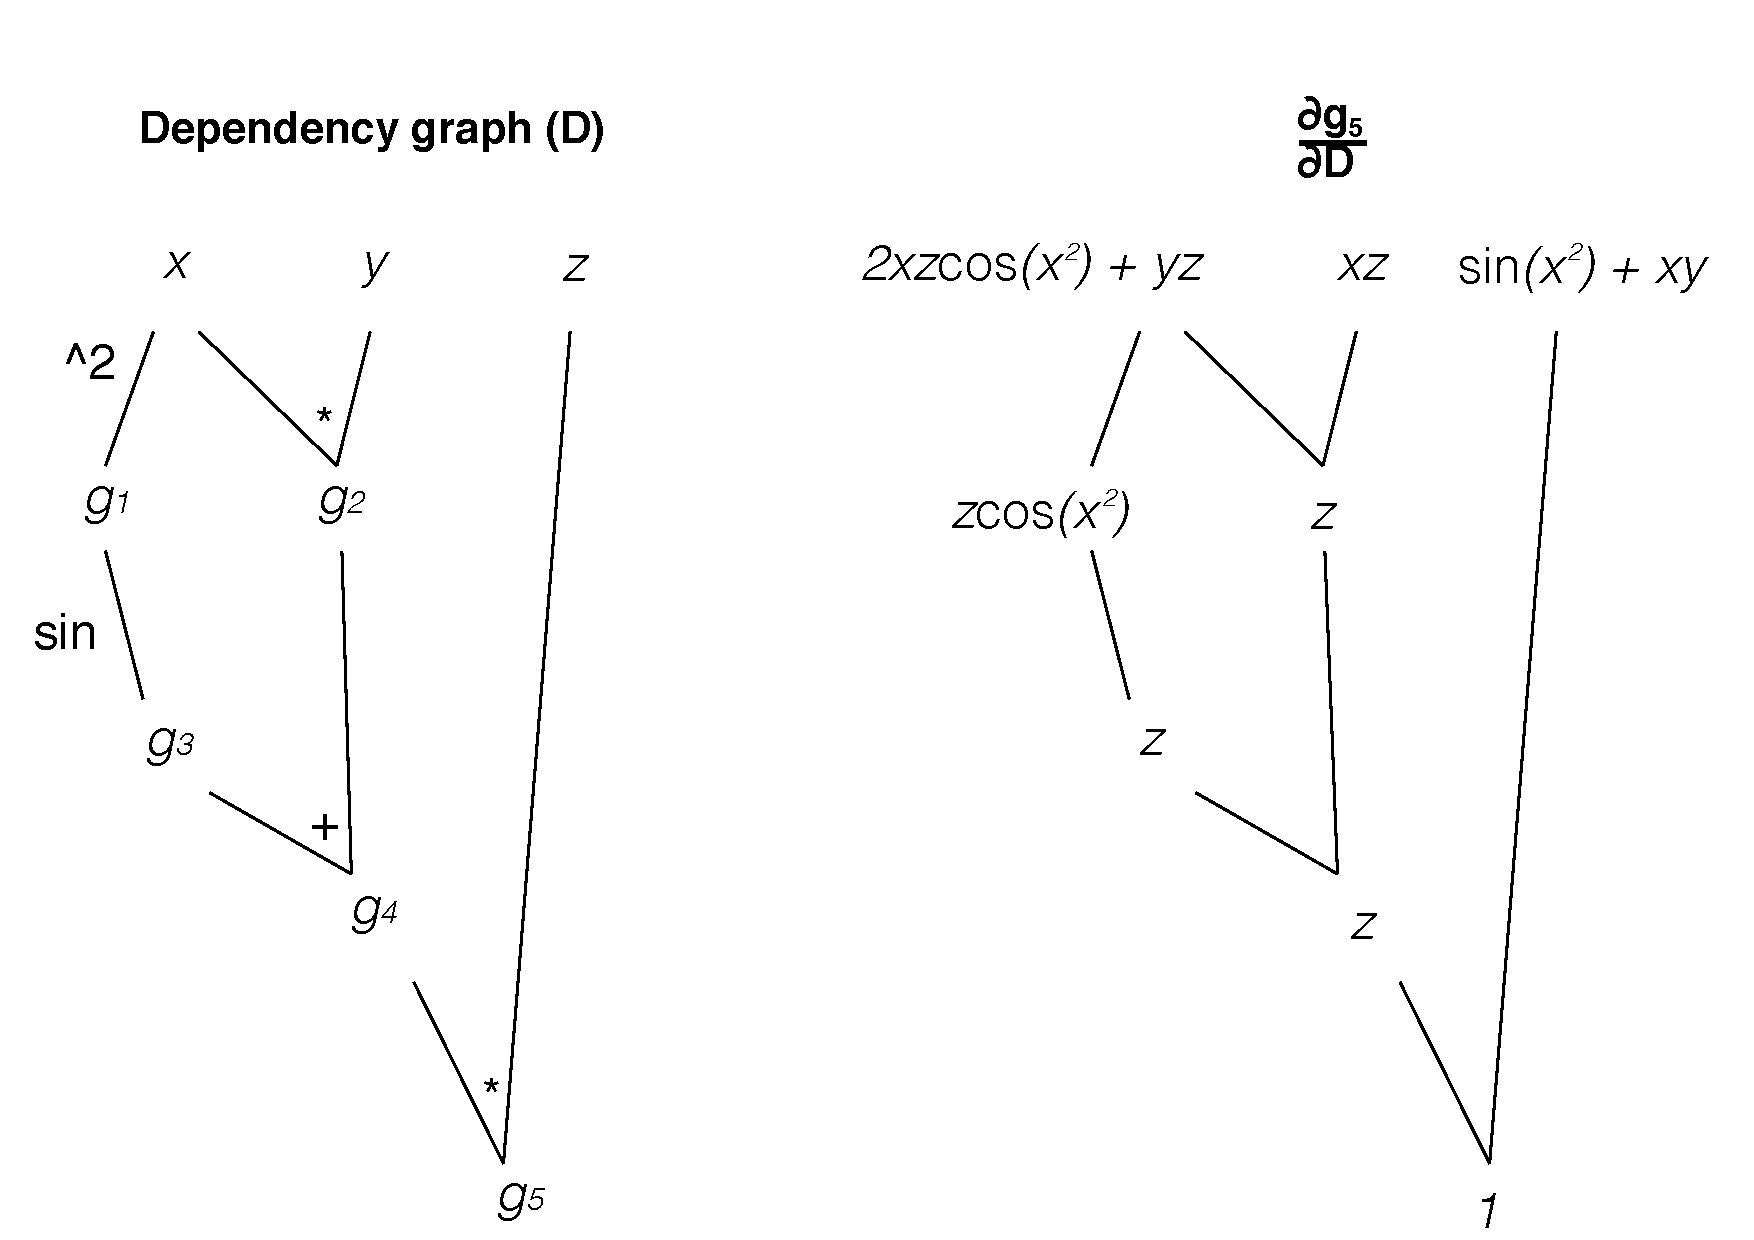
\includegraphics[width = 0.9\textwidth]{figures/dependency_graph_backward_AD.pdf}
 	    \caption{Graphs to visualize the process of backward AD. To the left is a dependency graph of the elementary functions in \eqref{eq:DependencyBackwardAD} and to the right are the derivatives of $g_5$ with respect to the dependencies given in the dependency graph.}
	\label{fig:depency_graph_backward_AD}
\end{figure}
Comparing this to the method of dual numbers from \autoref{sec:DualNumbers}, where we would have to evaluate $f$ three times, once for each derivative, this is a big improvement. This illustrates the strength of backward AD -- no matter how many input parameters a function have, you only need one function evaluation to get all the derivatives of the function. 
The disadvantage of backward AD is that to be able carry along function and derivative values as we did in forward AD, we need to implement the dependency tree shown in \autoref{fig:depency_graph_backward_AD}. This makes the implementation of backward AD much harder than for forward AD, and an inefficient implementation of this tree will reduce the advantage of backward AD. Also, if $f$ is a vector-evaluated function $f: \Re^n \rightarrow \Re^m$ and not a scalar function, backward AD needs to run $m$ times. Hence, if $n\approx m$, forward AD and backward AD will have approximately the same complexity. This is the main reason why we in the following will focus on implementing forward rather than backward AD.

\subsection{Forward Automatic Differentiation With Multiple Parameters}
\label{sec:FADWithMultipleParameters}
When we are dealing with functions with many input parameters and we wish to implement a forward AD, there are alternative ways of implementing this, rather than implementing with dual numbers and evaluating the function $n$ times.  \citet{doi:10.1137/080743627} describes a method that calculates all the derivatives in one function evaluation. To illustrate this method, consider a scalar function $f: \Re^n \rightarrow \Re$, that we want to obtain the gradient of. Then, the main idea is that we define what we call our \textit{primary variables}. This is all the variables in the space that we are currently working in. Each primary variable is an AD-variable containing the derivatives of itself with respect to all the other primary variables. Say we have three variables $x$, $y$ and $z$, and for any function $f(x,y,z)$ we are interested in finding the gradient of $f$, $\nabla f=(f_x, f_y, f_z)^\top$. To achieve this, we define the corresponding AD-variables
\begin{equation*}
    [\adpair{x}{(1,0,0)^\top}]\hspace{2em},\hspace{2em}
    [\adpair{y}{(0,1,0)^\top}]\hspace{2em},\hspace{2em}
    [\adpair{z}{(0,0,1)^\top}].
\end{equation*}
Each primary AD-variable now not only stores its derivative with respect to itself, but also the gradient with respect to all other primary variables. The operators defined in (\ref{eq:arithmeticOperators}) and the elementary functions in (\ref{eq:elementaryFunctions}) are still valid, except that scalar products are now vector products. As an example, let $f(x,y,z) = xyz$ and $x = 1$, $y = 2$ and $z = 3$, then
\begin{align*}
    xyz &= [\adpair{1}{(1,0,0)^\top}]\cdot [\adpair{2}{(0,1,0)^\top}]\cdot
    [\adpair{3}{(0,0,1)^\top}] \\
    &=[\adpair{1\cdot 2\cdot 3}{2\cdot3\cdot(1,0,0)^\top + 1\cdot3\cdot(0,1,0)^\top + 1\cdot2\cdot(0,0,1)^\top}] \\
    [\adpair{f}{\nabla f}] &= [\adpair{6}{(6,3,2)^\top}].
\end{align*}
This result is equal to the tuple
\begin{equation*}
    \big(f(x,y,z) \hspace{0.5em},\hspace{0.5em} \nabla f(x,y,z)\big) = \big(xyz ,\hspace{0.5em} (yz,xz,xy)^\top\big)
\end{equation*}
for the corresponding $x$, $y$ and $z$ values. 
\subsection{Forward Automatic Differentiation With Vector Functions}
\label{sec:FADWithVectorParameters}
For numerical solution of (partial) differential equations, the functions we evaluate as part of the discretization are usually vector functions and not scalar functions. Hence $f: \Re^n \rightarrow \Re^m$. Neidinger's method still applies, only that the primary variables are now vectors and instead of containing the gradient of itself with respect to all the other primary variables, we now have the Jacobian. For a function $f$, the Jacobian with respect to its $n$ primary variables is given as
\begin{align*}
    J_f  =
    \begin{pmatrix}
        \frac{\partial f_1}{\partial x_1} & \dotsb & \frac{\partial f_1}{x_n}\\
        \vdots & \ddots & \vdots \\
        \frac{\partial f_m}{\partial x_1} & \dotsb & \frac{\partial f_m}{x_n}
    \end{pmatrix}.
\end{align*}
The forward AD method described earlier will be similar for a vector function as it was for a scalar function. However, going from scalar functions with multiple parameters to vector functions induce two important differences. The first is that the primary variables need to be initialized with their Jacobians, and not just with a gradient vector. The Jacobian for a primary variable of dimension $n$ is the $n \times n$ identity matrix. The second change is that when evaluating new functions depending on the primary variables, the Jacobians corresponding to the functions will be calculated with matrix multiplication instead of the vector multiplication seen in the previous example. As a simple illustration of the differences, consider the vector function $f = 2\cdot \textbf{x}\cdot \textbf{y}$ for primary variables $\textbf{x},\textbf{y}\in \Re^3$ (we only consider element-wise multiplication). Initialization of the primary variables gives
\begin{equation}
    \label{def:VectorAD}
    \textbf{x} = \left[\adpair{\begin{pmatrix}1\\2\\3
    \end{pmatrix}}{\begin{pmatrix}
    1&0&0&0&0&0\\
    0&1&0&0&0&0\\
    0&0&1&0&0&0\end{pmatrix}} \right],
    \hspace{5em}
    \textbf{y} = \left[\adpair{\begin{pmatrix}4\\5\\6
    \end{pmatrix}}{\begin{pmatrix}
    0&0&0&1&0&0\\
    0&0&0&0&1&0\\
    0&0&0&0&0&1\end{pmatrix}} \right].
\end{equation}
Here, we have decided an order of the variables in the Jacobian, and further on, we need to be consistent with this order. The function value of $\textbf{x}\cdot\textbf{y}$ is found by normal element-wise multiplication. The Jacobian of $\textbf{x}\cdot\textbf{y}$ is obtained by using the chain rule as defined in \eqref{eq:arithmeticOperators}. The difference is now that we have \emph{element-wise} multiplication of a vector and a matrix instead of only scalars or scalars and vectors. Element-wise multiplication corresponds to transforming the vector to an $n\times n$ matrix with the values on the diagonal. The calculations give
\begin{align*}
    \textbf{x}\cdot\textbf{y} &= \left[\adpair{\begin{pmatrix}
        1\\2\\3
        \end{pmatrix}
        \cdot
        \begin{pmatrix}
        4\\5\\6
        \end{pmatrix}
    }{
        \begin{pmatrix}
        4&0&0\\
        0&5&0\\
        0&0&6\end{pmatrix}
        \cdot
        \begin{pmatrix}
        1&0&0&0&0&0\\
        0&1&0&0&0&0\\
        0&0&1&0&0&0
        \end{pmatrix}
        +
        \begin{pmatrix}
        1&0&0\\
        0&2&0\\
        0&0&3
        \end{pmatrix}
        \cdot
        \begin{pmatrix}
        0&0&0&1&0&0\\
        0&0&0&0&1&0\\
        0&0&0&0&0&1
        \end{pmatrix}}\right]
        \\
        &= \left[\adpair{
        \begin{pmatrix}
        4\\10\\18
        \end{pmatrix}
        }{
        \begin{pmatrix}
        4&0&0&1&0&0\\
        0&5&0&0&2&0\\
        0&0&6&0&0&3
        \end{pmatrix}
        }\right].
\end{align*}
Finally, the expression for the vector function $f$ is found by observing that element-wise multiplication between a scalar and an AD-variable corresponds to multiplying every element in that AD-variable with the scalar. This gives
\begin{align*}
    f = \left[\adpair{
        \begin{pmatrix}
        8\\20\\36
        \end{pmatrix}
        }{
        \begin{pmatrix}
        8&0&0&2&0&0\\
        0&10&0&0&4&0\\
        0&0&12&0&0&6
        \end{pmatrix}
        }\right].
\end{align*}
\section{Applications of Automatic Differentiation}
\label{sec:ApplicationsAD}
AD can be used in a wide specter of applications; common for many of them is that we have a vector or scalar function we want to minimize or find the roots of. This section considers some of the applications where AD can be used -- from solving simple linear systems to solving the Poisson equation with discrete divergence and gradient operators.

\subsection{The Newton-Raphson Method}
The simplest example for finding roots is for a scalar function $f$ with a scalar input $x$. Then the Newton--Raphson method
\begin{equation*}
    x_{i+1} = x_i - \frac{f(x_i)}{f'(x_i)},
\end{equation*}
for an initial $x_0$, will converge to a root of $f$ given that $f$ is sufficiently smooth. With AD, this is quite simple to implement, as you only have to define the function $f(x)$, and then AD finds $f'(x)$ automatically. You can then use the Newton-Raphson method directly. Exactly the same approach can be used to solve nonlinear systems in multiple dimensions. As a simple illustration, let us look at the \emph{linear} system 
\begin{equation}
    \textbf{A}\boldsymbol{x} = \textbf{b},
    \label{eq:linearSystem}
\end{equation}
which we can write on residual form such that
\begin{equation*}
	\boldsymbol{F}(\boldsymbol{x}) = \textbf{A}\boldsymbol{x} - \boldsymbol{b} = 0 .
\end{equation*}
This means that to solve the linear system in \myeqref{eq:linearSystem}, we need to find the root of $\boldsymbol{F}(\boldsymbol{x})$. This can be done by choosing an initial value $\boldsymbol{x}^0$ and observe that since $\boldsymbol{F}(\boldsymbol{x})$ is linear, the corresponding multivariate Newton-Raphson method will converge in one step. The general form of the multivariate Newton-Raphson method is given by
\begin{equation}
	\boldsymbol{x}^{n+1} = \boldsymbol{x}^n - J_{\boldsymbol{F}}  (\boldsymbol{x}^n)^{-1} \boldsymbol{F}(\boldsymbol{x}^n).
    \label{eq:newtonRaphsonVector}
\end{equation}
Here, $J_{\boldsymbol{F}}  (\boldsymbol{x}^n)^{-1}$ is the inverse of the Jacobian of $\boldsymbol{F}$ at $\boldsymbol{x}^n$. 

\subsection{Solving the Poisson Equation}
\label{sec:poissonEq}
For a simple linear system like \myeqref{eq:linearSystem} it may seem a bit forced and unnecessary to make the effort of using AD to solve for $\boldsymbol{x}$. We could just as well have used some built in linear solver. But for applications to the numerical solution of partial differential equations (PDEs), this approach greatly simplifies the process of (linearizing and) assembling the linear systems that appear when you solve the (non)linear system of discretized equations. Indeed, using \myeqref{eq:newtonRaphsonVector} with AD, all you have to do is implement the discretized equations on residual form.  As a preface to introducing how we will do this, we consider the Poisson equation
\begin{equation}
    -\nabla(\textbf{K}\nabla u) = q,
    \label{eq:Poisson}
\end{equation}
where \textbf{K} is a spatially variable coefficient, and we want to find $u$ on the domain $\Omega \in \Re^d$. Numerically, this can be done by using a finite volume method. This approach is based on applying conservation laws inside the domain. By dividing the domain into a grid of smaller cells, $\Omega_i$, we can instead of looking at the Poisson equation in differential form, integrate it over each cell such that
\begin{equation}
    \int_{\partial\Omega_i}\!\!- \textbf{K} \nabla u \cdot \textbf{n}\, \mbox{ds} = \int_{\Omega_i} q \,\mbox{dA}.
    \label{eq:conservation}
\end{equation}
Here, \textbf{n} is the unit normal to the cell $\Omega_i$, so \myeqref{eq:conservation} describes the conservation of mass in the cell $\Omega_i$, where total flux in and out of the boundary of $\Omega_i$ is equal to the total accumulation from source and sink terms inside $\Omega_i$. For simplicity, we define $\textbf{v} = - \textbf{K} \nabla u$ as the flux. As a simple example to begin with, we will consider \autoref{fig:gridTwoCells}, which shows two cells $\Omega_i$ and $\Omega_k$. The average values of $u$ inside the two cells are $u_i$ and $u_k$, and the interface, or facet, between the cells is defined as $\Gamma_{i,k}$.
\begin{figure}[H]
    \centering
    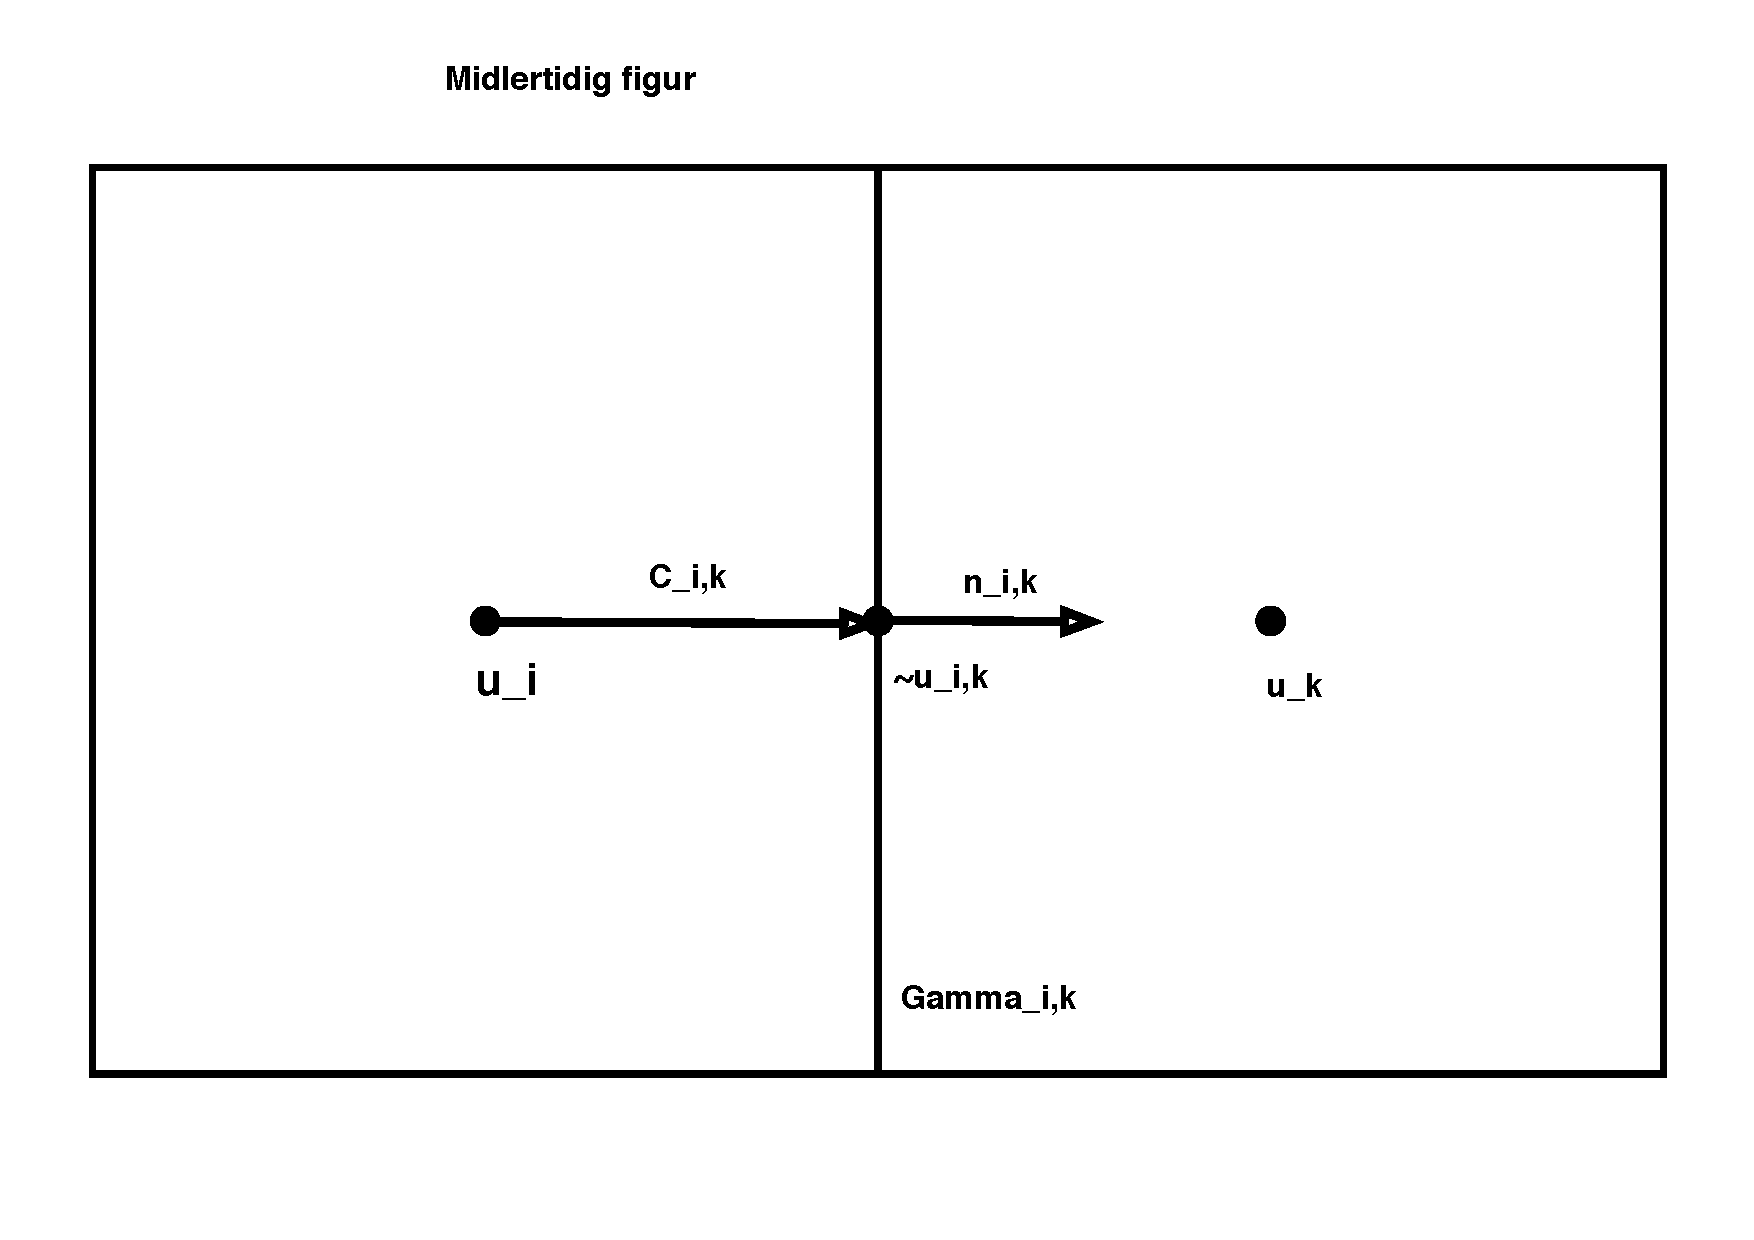
\includegraphics[width = 0.7\textwidth]{figures/grid_two_cells.pdf}
    \caption{Figure of two adjacent cells $\Omega_i$ and $\Omega_k$. The average value of the cell is given by $u_i$. The boundary between the cells is $\Gamma_{i,k}$ with value at the centre equal $\tilde{u}_{i,k}$ and outward normal vector $n_{i,k}$}
    \label{fig:gridTwoCells}
\end{figure}
Now, the flux through the common interface $\Gamma_{i,k}$ can be computed by
\begin{equation}
    v_{i,k} = \int_{\Gamma_{i,k}} \textbf{v}\cdot\textbf{n}_{i,k} \mbox{ds}. 
    \label{eq:fluxOverBoundary}
\end{equation}
The integral in \eqref{eq:fluxOverBoundary} can be approximated by the midpoint rule with $\tilde{\textbf{v}}_{i,k}$ as the flux on the midpoint of $\Gamma_{i,k}$. If we let $L_{i,k}$ be the length of $\Gamma_{i,k}$, then 
\begin{equation*}
    v_{i,k} \approx L_{i,k}\tilde{\textbf{v}}_{i,k} \cdot \textbf{n}_{i,k} = -L_{i,k}\textbf{K}\nabla \tilde{u}_{i,k} \cdot \textbf{n}_{i,k}.
\end{equation*}
Here, $\tilde{u}_{i,k}$ is the value of $u$ at the centre of the facet $\Gamma_{i,k}$. The problem we now face is that in the finite volume method, we only know the average value of $u$ over each cell. If we use a first-order reconstruction, the reconstructed value at the center of cell $\Omega_i$ coincides with the average value $u_i$. Assuming the underlying function is sufficiently smooth, we can then use a finite-difference method to approximate the gradient of $u$ on $\Gamma_{i,k}$, expressed in terms of the value $u_i$ at the cell center and the value $\tilde{u}_{i,k}$ at the midpoint of the facet,
\begin{equation*}
    v_{i,k} \approx L_{i,k}\textbf{K}_i\frac{(\tilde{u}_{i,k} - u_i)\textbf{c}_{i,k}}{|\textbf{c}_{i,k}|^2} \cdot \textbf{n}_{i,k}.
\end{equation*}
Here, $\textbf{c}_{i,k}$ is the vector from $u_i$ to $\tilde{u}_{i,k}$ as seen in \autoref{fig:gridTwoCells}.  For brevity, we collect all the known quantities into a scalar quantity, which we call the transmissibility,
\begin{equation}
    T_{i,k} = L_{i,k}\textbf{K}_i\frac{\textbf{c}_{i,k}}{|\textbf{c}_{i,k}|^2} \cdot \textbf{n}_{i,k}.
    \label{eq:transmissibility}
\end{equation}
Because we know that the amount of flux from cell $\Omega_i$ to $\Omega_k$ must be the same as from $\Omega_k$ to $\Omega_i$, only with opposite sign, we have the relation $v_{i,k} = -v_{k,i}$.  In most cases, we will also have continuity across the interface, so that $\tilde{u}_{i,k} = \tilde{u}_{k,i}$. Hence, we have the relation 
\begin{equation*}
    v_{i,k} = T_{i,k}(\tilde{u}_{i,k} - u_i) \hspace{3em} -v_{i,k} = T_{k,i}(\tilde{u}_{i,k} - u_k).
\end{equation*}
By subtracting the two equations for $v_{i,k}$ and moving $T_{i,k}$ and $T_{k,i}$ to the other side 
\begin{equation}
    \begin{aligned}
        (T_{i,k}^{-1} + T_{k,i}^{-1}) v_{i,k} &= (\tilde{u}_{i,k} - u_i) - (\tilde{u}_{i,k} - u_k)
        \\
        v_{i,k} &= (T_{i,k}^{-1} + T_{k,i}^{-1})^{-1}(u_k - u_i) = T_{ik}(u_k - u_i)
    \end{aligned}
    \label{eq:flux}
\end{equation}
we manage to eliminate $\tilde{u}_{i,k}$ and get a computable expression for the gradient of $u$. This is called the two-point flux-approximation (TPFA) \citep{lieMrstUrl}. Now that we have an approximation of the flux through the interface between $\Omega_i$ and $\Omega_k$, we get that \myeqref{eq:fluxOverBoundary} can be approximated by 
\begin{equation}
    \sum_k T_{i,k}(u_k - u_i) = q_i, \hspace{3em} \forall \Omega_i \in \Omega,
    \label{eq:PoissonSolvableTwoCells}
\end{equation}
where $q_i$ is the integrated accumulation over cell $\Omega_i$. Now, we can get a linear system of the form \textbf{A}\textbf{u} = \textbf{b},  which on residual form becomes \textbf{F}(\textbf{u}) = \textbf{A}\textbf{u} - \textbf{b} = 0 where
\begin{align*}
    \textbf{A}_{i,j} = 
    \left\lbrace
    \begin{array}{lr}
    \sum_k T_{ik} \hspace{3em}&\text{if } j = i\\
    -T_{ij} \hspace{3em}&\text{if } j \neq i.
    \end{array}
    \right.
\end{align*}
This means we can solve the Poisson \myeqref{eq:Poisson}, using the scheme explained in \eqref{eq:newtonRaphsonVector} and by having $u$ as an AD-variable. For this simple Poisson equation, we still only end up with a linear system of equations that we may as well solve without AD. The only benefit is that we never need to form the matrix $\mathbf{A}$ explicitly, which can be bit complicated for more complex grids. For nonlinear PDEs, we would also need to linearize the local discrete equations, and the construction of the matrix \textbf{A} generally becomes more tricky.  The ease of using AD becomes clearer when we combine it with discrete differentiation operators that we will define in the next subsection.

\subsection{Discrete Differentiation Operators}
\label{sec:DiscreteOperators}
To show the real elegance of using AD to solve PDEs, we want to create a framework in which we have defined discrete divergence and gradient operators such that we can write the discrete equations we want to solve on a similar form as in the continuous case. We also want to be able to do this no matter how complex and unstructured our grid is.

Instead of the simple two-cell grid we used in \autoref{fig:gridTwoCells}, we now consider a a general polygonal grid. \autoref{fig:partialGrid} illustrates an example, in which all cells are quadrilaterals. To define the discrete divergence and gradient operators, we need some information about the topology of the grid. The grid can be described in terms of three types of objects: cells, facets and vertices. The cells are each $\Omega_i \subset \Omega$. In our two-dimensional case, the facets are simply the lines that delimit each cell, and the vertices are the endpoints of each facet. In addition, we introduce nodes. In the case demonstrated by \autoref{fig:gridTwoCells}, we had two nodes, $u_i$ and $u_k$, and for the finite-volume method they are the average value of $u$ on the corresponding cell. Each cell and facet has physical properties like area or length, and centroid or centre. Each facet also has a normal vector. 
\begin{figure}[H]
    \centering
    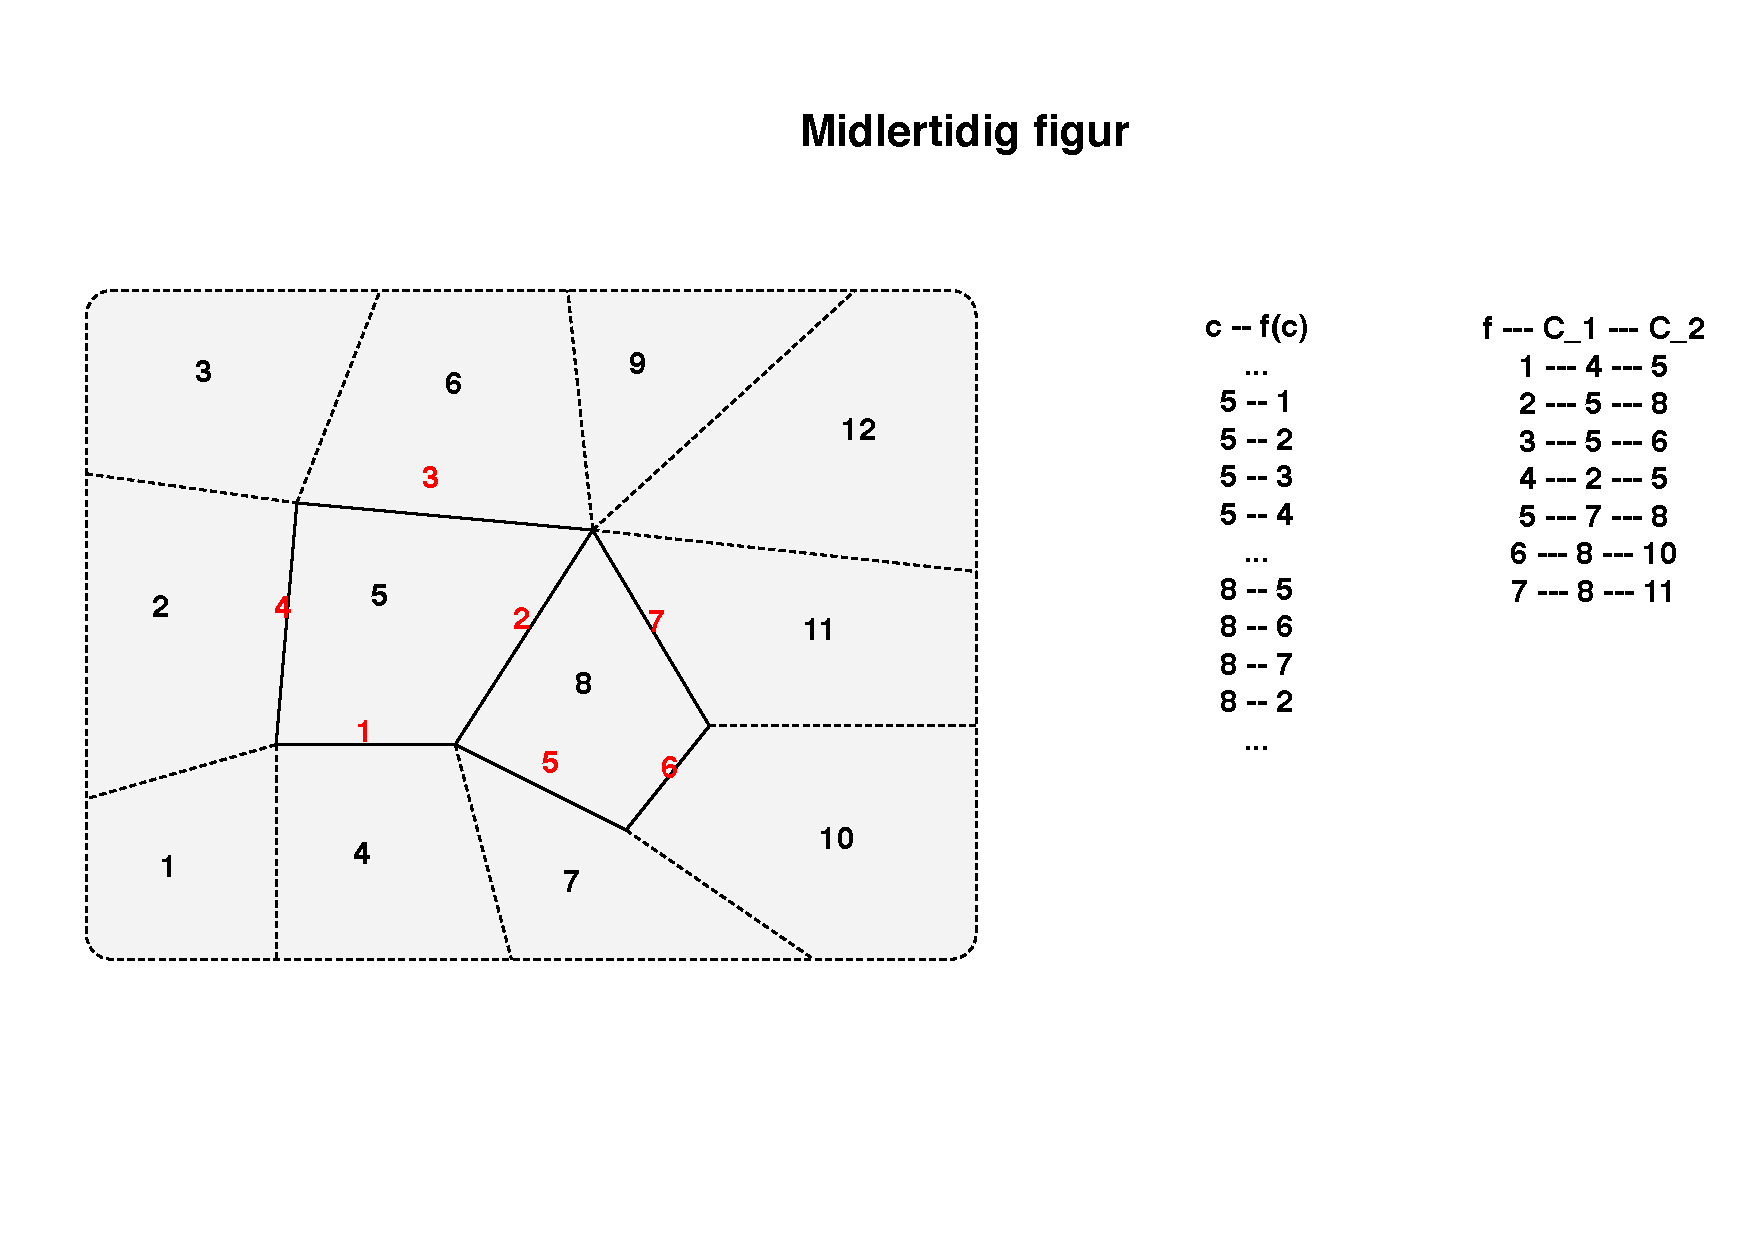
\includegraphics[width = 0.7\textwidth]{figures/grid_cells_facets.pdf}
    \caption{Figure of a general polygonal grid with the mapping cell to facets and facet to cells.}
    \label{fig:partialGrid}
\end{figure}

\autoref{fig:partialGrid} shows how we can introduce two different mappings that explain the relation between the cells and the facets. The mappings for cells 5 and 8 are written out. The first relation, $F(c)$, is the mapping from cells $c$ to their delimiting facets $f$. The second mapping, $C_i(f)$ for $i = 1,2$, is a mapping from a facet $f$ to the two cells $C_1$ and $C_2$ that share this facet. All these properties will be used to create the discrete divergence and gradient operators.

We now have all the physical properties of the grid we used to attain the formulae in \myeqref{eq:PoissonSolvableTwoCells}. From these, we want to create discrete divergence and gradient operators that correspond to the continuous equivalents for this grid. Consider the Poisson \myeqref{eq:Poisson} for the function $u$. Then the discrete gradient operator for a facet $f$ is defined as 
\begin{equation}
    \texttt{dGrad}(u)[f] = u[C_2(f)] - u[C_1(f)], 
    \label{eq:discreteGradient}
\end{equation}
where $u[C_i(f)]$ is the value of $u$ at the cell corresponding to $C_i(f)$. For the divergence operator, we remember the expression we found for the flux through a facet in \myeqref{eq:flux}. Let $v_{i,k} = v[f]$, where $f$ is the facet between cell $i$ and cell $k$. Since the divergence in a cell is the same as the sum of flux leaving and entering the cell, the discrete divergence operator for cell $c$ is defined as 
\begin{equation*}
    \texttt{dDiv}(\textbf{v})[c] = \sum_{f\in f(c)} \operatorname{sgn}(f)v[f]
\end{equation*}
where the function $\operatorname{sgn}(f)$ is defined as 
\begin{align*}
    \text{sgn}(f) = \left\lbrace
    \begin{array}{rl}
        1 \hspace{3em}&\text{if } c \in C_1(f)\\
        -1 \hspace{3em}&\text{if } c \in C_2(f).
    \end{array}
    \right.
\end{align*}
The discrete operators $\texttt{dDiv}$ and $\texttt{dGrad}$ can be represented in terms of sparse matrices that are simple to form from the mappings $F$ and $C_1,C_2$; see \cite{lieMrstUrl} for more details.

The extra \texttt{d} in front of the names stands for discrete and is included so that we later avoid name collision with Julia's built in \texttt{div} function. Now we can create discrete divergence and gradient operators, only based on the topology of the grid, so that the discrete Poisson equations we want to solve can be written very similar to the continuous case
\begin{align*}
    -\nabla(\textbf{K}\nabla u) - q &= 0 \qquad \longleftrightarrow\qquad
    \textbf{F}(\textbf{u}) = \texttt{dDiv}(\textbf{T }\texttt{dGrad}(\textbf{u}))-\textbf{q} 
    = 0.
\end{align*}
Here, \textbf{T} is the transmissibility defined in \eqref{eq:transmissibility}. The notation for the discrete equations is clearly similar to the continuous case, and we can actually read the discrete expression and directly understand what equation we are trying to solve. For this simple Poisson equation, we will still have a linear system and we would not necessarily need to use AD to solve it. But for more complex problems, we can derive the discrete divergence and gradient operators in the same approach for any type of grid. Although the system then becomes non-linear, it will be easy to solve using AD and the Newton-Raphson method. An example of this can be seen in \autoref{ch:FlowSolver}.
